% ICASSP 2026 paper draft for the low-resource ASR project.
\documentclass{article}
\usepackage{spconf,amsmath,graphicx,booktabs,array,url,tikz}
\usetikzlibrary{arrows.meta,positioning}

\title{LOW-RESOURCE ENGLISH ASR WITH CONTINUOUS WAV2VEC 2.0 REPRESENTATIONS}
\name{Author Name(s)}
\address{Course Project, Institution Name}

\begin{document}
\maketitle

\begin{abstract}
This paper presents a low-resource English automatic speech recognition (ASR) baseline based on self-supervised speech representations. We build a character-level CTC recognizer on top of the pretrained wav2vec 2.0 Base encoder and evaluate it on small subsets of LibriSpeech. To quantify the value of adapting the self-supervised encoder, we compare two systems under the same data and vocabulary settings: a frozen-encoder baseline that trains only the randomly initialized CTC head, and a fine-tuned system that updates the Transformer encoder while keeping the convolutional feature extractor frozen. On a 10\% LibriSpeech test subset after training with 1\% of train-clean-100, fine-tuning reduces WER from 99.55\% to 25.73\% and CER from 69.98\% to 7.47\%. Error analysis shows that the fine-tuned model mainly makes phonetically plausible spelling and word-boundary errors, whereas the frozen baseline often produces empty or unreadable character fragments.
\end{abstract}

\begin{keywords}
low-resource ASR, self-supervised speech representation, wav2vec 2.0, CTC, LibriSpeech
\end{keywords}

\section{Introduction}
\label{sec:intro}

Low-resource automatic speech recognition requires learning an acoustic-to-text mapping from limited transcribed speech. Self-supervised speech models address this constraint by pretraining on large unlabeled speech corpora and providing contextual acoustic representations that can be adapted to downstream ASR tasks. wav2vec 2.0 is a representative approach that learns latent speech representations with a contrastive objective and has been widely used as an ASR encoder \cite{baevski2020wav2vec}.

This project studies how effectively continuous self-supervised representations support low-resource English ASR. We implement a compact and reproducible baseline using wav2vec 2.0 Base and a CTC output layer \cite{graves2006ctc}. The main comparison is between freezing the pretrained encoder and fine-tuning it with limited labeled data. This comparison isolates whether the pretrained representation is directly linearly separable enough for character recognition or whether supervised adaptation of the encoder is required.

The contribution is threefold: (1) a complete low-resource ASR pipeline using LibriSpeech, wav2vec 2.0, CTC training, and WER/CER evaluation; (2) a controlled frozen-versus-fine-tuned comparison; and (3) an error analysis that contrasts local spelling errors with complete decoding failures.

\section{System Design}
\label{sec:method}

\subsection{Task and data setting}

The task is English speech-to-text transcription. We use the Hugging Face version of LibriSpeech ASR \cite{panayotov2015librispeech} with the clean configuration. To simulate a low-resource condition, the training split is restricted to \texttt{train.100[:1\%]}. Validation and test evaluation use \texttt{validation[:10\%]} and \texttt{test[:10\%]}, respectively.

All audio is resampled to 16 kHz by the dataset audio pipeline. Transcripts are normalized to lowercase letters, spaces, and apostrophes. For CTC training, spaces are represented by the word delimiter token ``\texttt{|}'', and the character vocabulary is built automatically from the training transcripts.

\subsection{Model architecture}

Both systems use \texttt{facebook/wav2vec2-base} as the speech self-supervised encoder. A randomly initialized linear CTC classification head maps encoder states to character labels. Given input waveform $x$ and target character sequence $y$, training minimizes the CTC loss
\begin{equation}
  \mathcal{L}_{\mathrm{CTC}} = -\log p(y \mid x),
\end{equation}
which marginalizes over all frame-level alignments compatible with the target transcription.

We evaluate two parameter-update strategies. The frozen baseline freezes the entire wav2vec 2.0 base model and trains only the CTC head. The fine-tuned system freezes only the convolutional feature extractor and updates the Transformer encoder together with the CTC head. This design keeps the front-end acoustic feature extractor stable while allowing contextual representations to adapt to the ASR objective.

\begin{figure}[t]
\centering
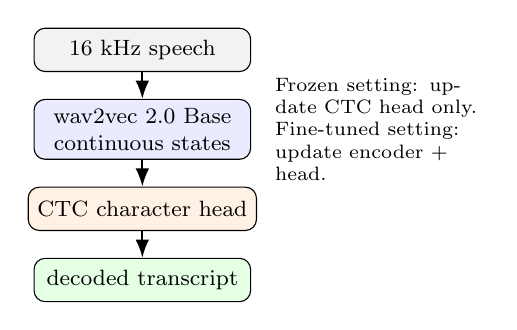
\begin{tikzpicture}[
  node distance=0.34cm,
  box/.style={draw, rounded corners, align=center, minimum width=2.75cm,
              minimum height=0.55cm, font=\footnotesize},
  arrow/.style={-Latex, thick}
]
\node[box, fill=gray!10] (audio) {16 kHz speech};
\node[box, fill=blue!8, below=of audio] (ssl) {wav2vec 2.0 Base\\continuous states};
\node[box, fill=orange!10, below=of ssl] (ctc) {CTC character head};
\node[box, fill=green!10, below=of ctc] (text) {decoded transcript};
\draw[arrow] (audio) -- (ssl);
\draw[arrow] (ssl) -- (ctc);
\draw[arrow] (ctc) -- (text);
\node[align=left, font=\scriptsize, right=0.18cm of ssl, text width=2.6cm]
  {Frozen setting: update CTC head only.\\Fine-tuned setting: update encoder + head.};
\end{tikzpicture}
\caption{System overview. The project uses continuous wav2vec 2.0 hidden states and CTC decoding for low-resource ASR.}
\label{fig:pipeline}
\end{figure}

\section{Experimental Setup}
\label{sec:setup}

The experiments are implemented with PyTorch and Hugging Face Transformers \cite{wolf2020transformers}. Training uses mixed precision on a single GPU. The frozen baseline is trained with batch size 2, learning rate $10^{-3}$, and 400 optimization steps. The fine-tuned model uses batch size 2, gradient accumulation over 8 steps, learning rate $10^{-4}$, 100 warmup steps, and 800 optimization steps. The fine-tuned model uses gradient checkpointing to reduce memory usage.

We report word error rate (WER) and character error rate (CER), the standard edit-distance based ASR metrics. Lower values indicate better recognition accuracy. We also report the number of trainable parameters to show the difference in optimization capacity between the two settings.

\section{Results and Analysis}
\label{sec:results}

\subsection{Recognition accuracy}

Table~\ref{tab:main_results} shows the main results. Freezing the wav2vec 2.0 encoder gives nearly unusable recognition quality: test WER is 99.55\% and test CER is 69.98\%. Although the pretrained encoder contains rich acoustic information, the randomly initialized CTC head alone is not sufficient to learn a reliable character mapping from the small labeled subset.

Fine-tuning the encoder dramatically improves recognition. Test WER decreases to 25.73\%, and test CER decreases to 7.47\%. The improvement indicates that downstream supervision must reshape the continuous SSL representations for ASR, especially when the output vocabulary and CTC alignment objective are newly introduced.

\begin{figure}[t]
\centering
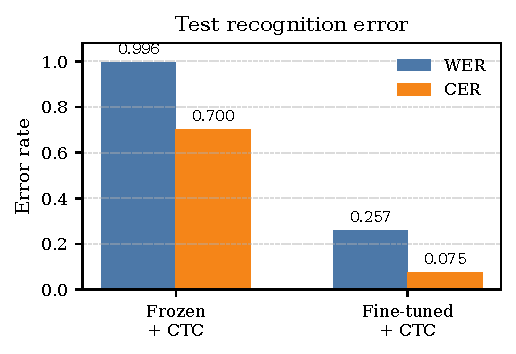
\includegraphics[width=0.98\linewidth]{figures/wer_cer_bars.pdf}
\caption{Test WER and CER for the frozen and fine-tuned wav2vec 2.0 systems. Fine-tuning substantially improves both word-level and character-level accuracy.}
\label{fig:wer_cer}
\end{figure}

\begin{table}[t]
\centering
\caption{Low-resource LibriSpeech ASR results. The training split is \texttt{train.100[:1\%]}; validation and test splits use 10\% subsets.}
\label{tab:main_results}
\resizebox{\linewidth}{!}{%
\begin{tabular}{lrrrrr}
\toprule
System & Trainable & Eval WER & Eval CER & Test WER & Test CER \\
\midrule
Frozen + CTC & 24.6K & 0.9965 & 0.7308 & 0.9955 & 0.6998 \\
Fine-tuned + CTC & 90.2M & 0.2917 & 0.0847 & 0.2573 & 0.0747 \\
\bottomrule
\end{tabular}
}
\end{table}

\begin{figure}[t]
\centering
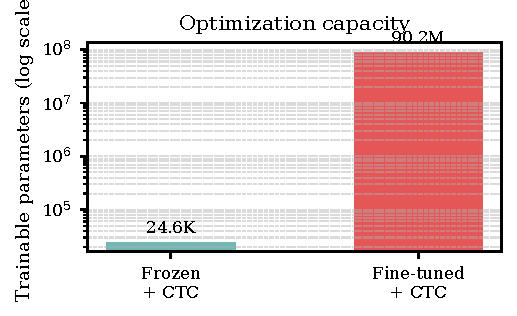
\includegraphics[width=0.9\linewidth]{figures/trainable_params.pdf}
\caption{Trainable parameter counts for the two update strategies. The fine-tuned system has much larger optimization capacity because the Transformer encoder is updated.}
\label{fig:params}
\end{figure}

\subsection{Error analysis}

Table~\ref{tab:error_examples} lists representative test examples. The fine-tuned system usually preserves sentence structure and produces phonetically plausible errors, such as \textit{agitated} becoming \textit{agetated} or \textit{beckon} becoming \textit{beckeon}. Some errors are caused by punctuation normalization, e.g., missing apostrophes in \textit{you'd}. Short utterances and proper names remain challenging, as seen in \textit{hans stirs not}.

In contrast, the frozen baseline often outputs empty strings or very short character fragments. These errors are not merely word substitutions; they indicate that the CTC head has not learned a stable mapping from frozen speech states to characters. This qualitative difference supports the quantitative gap in Table~\ref{tab:main_results}.

\begin{table*}[t]
\centering
\caption{Representative recognition errors from the test subset.}
\label{tab:error_examples}
\begin{tabular}{p{0.22\linewidth}p{0.36\linewidth}p{0.36\linewidth}}
\toprule
System / type & Reference & Prediction \\
\midrule
Fine-tuned spelling & yes i need repose many things have agitated me to day & yes i need repose many things have agetated me to day \\
Fine-tuned word ending & this and more will i dare in his service & this and more will i dare in his serviscs \\
Fine-tuned word boundary & if you'd rather not & if youd rather not \\
Fine-tuned short sentence & hans stirs not & haond sturs night \\
Frozen empty output & what was that & \\
Frozen fragment & tuesday august eighteenth & tt \\
Frozen unreadable output & each of us is lashed to some part of the raft & vslm \\
\bottomrule
\end{tabular}
\end{table*}

\subsection{Discussion}

The experiment focuses on continuous hidden-state representations rather than discrete speech units. This is an intentional baseline choice: continuous wav2vec 2.0 states can be connected directly to CTC and avoid additional clustering, codebook-size selection, token-rate measurement, and unit-to-text modeling. The limitation is that this system does not evaluate bitrate or codebook efficiency. A natural extension is to compare the current continuous representation with K-means or HuBERT-style discrete units, or to run the provided 5\% data configuration to measure the effect of labeled data scale.

\section{Conclusion}
\label{sec:conclusion}

We built and evaluated a low-resource English ASR baseline using wav2vec 2.0 continuous self-supervised representations and CTC training. The frozen-encoder system fails to produce reliable transcriptions, while fine-tuning the wav2vec 2.0 Transformer encoder reduces test WER from 99.55\% to 25.73\%. The results show that pretrained speech representations are highly useful for low-resource ASR, but effective use requires supervised adaptation rather than only training a shallow classification head. Future work should compare different SSL encoders, different representation layers, and discrete-unit variants under the same evaluation protocol.

\section{References}
\label{sec:refs}
\bibliographystyle{IEEEbib}
\bibliography{refs}

\end{document}
